\chapter{Matrices}

\begin{enumerate}
    \item With $m, n \in \mathbb{N}$ a real-valued $(m, n)$ matrix $\bm{A}$ is an $m\cdot n$-tuple of elements $a_{ij}$, $i = 1, \cdots , m$, $j = 1, \cdots , n$, which is ordered according to a rectangular scheme consisting of $m$ rows and $n$ columns:
    \\[0.2cm]
    $
        \bm{A}
        = 
        \begin{bmatrix}
            a_{11} & a_{12} & \cdots & a_{1n} \\
            a_{21} & a_{22} & \cdots & a_{2n} \\
            \vdots & \vdots & \ddots & \vdots \\
            a_{m1} & a_{m2} & \cdots & a_{mn} \\
        \end{bmatrix}
        \hfill
        (\ a_{ij} \in \mathbb{R} \ )
    $
    \hfill \cite{mfml/book/mml/Deisenroth-Faisal-Ong}

    \item $\mathbb{R}^{m\times n}$ is the set of all real-valued $(m, n)$-matrices. $\bm{A} \in \mathbb{R}^{m\times n}$ can be equivalently represented as $\bm{a} \in \mathbb{R}^{mn}$ by stacking all $n$ columns of the matrix into a long vector.
    \hfill \cite{mfml/book/mml/Deisenroth-Faisal-Ong}

    \vspace{0.5cm}

    \item They can be used to compactly represent systems of linear equations, but they also represent linear functions (linear mappings).
    \hfill \cite{mfml/book/mml/Deisenroth-Faisal-Ong}

    \item matrix represents a linear mapping or a collection of vectors.
    \hfill \cite{mfml/book/mml/Deisenroth-Faisal-Ong}
\end{enumerate}


\section{Matrix Operations}
\subsection{Matrix Addition ( $+$ )  \cite{mfml/book/mml/Deisenroth-Faisal-Ong}}

The sum of two matrices $\bm{A} \in \mbbR^{m\times n}$, $\bm{B} \in \mbbR^{m\times n}$ is defined as the element-wise sum:\\
. \hfill
\begin{customArrayStretch}{2}
$
    \bm{A} + \bm{B}
    := \begin{bmatrix}
        a_{11} + b_{11} &   \cdots  &  a_{1n} + b_{1n} \\
        \vdots          &   \ddots  &   \vdots  \\
        a_{m1} + b_{m1} &   \cdots  &  a_{mn} + b_{mn} \\
    \end{bmatrix}
    \in \mbbR^{m\times n}
$
\end{customArrayStretch}
\hfill \cite{mfml/book/mml/Deisenroth-Faisal-Ong}







\begin{lstlisting}[
    language=Python,
    caption=Matrix Addition - numPy
]
import numpy as np

m,n = 4,3

A = np.random.randint(-10, 10, size=(m,n))
B = np.random.randint(-10, 10, size=(m,n))

C = A + B

print("A:\n", A)
print("B:\n", B)
print("C:\n", C)
\end{lstlisting}









\subsection{Matrix Multiplication ( $AB$ OR $@$ OR $\cdot$ ) \cite{mfml/book/mml/Deisenroth-Faisal-Ong}}

For matrices $\bm{A} \in \mbbR^{m\times n}$, $\bm{B} \in \mbbR^{n\times k}$, the elements $c_{ij}$ of the product matrices. $\bm{C} = \bm{AB} \in \mbbR^{m\times k}$ are computed as:

\vspace{0.5cm}
\hfill
$
    c_{ij} = \dsum_{l=1}^n a_{il}\ b_{lj}
$
\hfill
$
    i = 1,\cdots,m
    \hspace{1cm}
    j = 1,\cdots,k
$
\hfill \cite{mfml/book/mml/Deisenroth-Faisal-Ong}





\begin{lstlisting}[
    language=Python,
    caption=Matrix Multiplication - numPy
]
import numpy as np

m,n,k = 4,3,5

A = np.random.randint(-10, 10, size=(m, n))
B = np.random.randint(-10, 10, size=(n, k))

C1 = A @ B
C2 = np.matmul(A, B)
C3 = np.dot(A, B)

print("A:\n", A)
print("B:\n", B)
print("C1:\n", C1)
print("C2:\n", C2)
print("C3:\n", C3)
print(np.all(C1 == C2), np.all(C1 == C3))
\end{lstlisting}




\vspace{0.5cm}

\begin{enumerate}
    \item To compute element $c_{ij}$ we multiply the elements of the $i$th row of $\bm{A}$ with the $j$th column of $\bm{B}$ and sum them up.
    \hfill \cite{mfml/book/mml/Deisenroth-Faisal-Ong}

    \item Matrices can only be multiplied if their “neighboring” dimensions match.
    \hfill \cite{mfml/book/mml/Deisenroth-Faisal-Ong}
    \\
    \hfill
    $
        \underset{n\times k}{\underbrace{\bm{A}}}\
        \underset{k\times m}{\underbrace{\bm{B}}}
        =
        \underset{n\times m}{\underbrace{\bm{C}}}
    $
    \hfill \cite{mfml/book/mml/Deisenroth-Faisal-Ong}
    \\
    The product $\bm{BA}$ is not defined if $m \neq n$ since the neighboring dimensions do not match.

    \item Matrix multiplication is \textbf{not} defined as an element-wise operation on matrix elements, i.e.,
    \\
    $c_{ij} \neq a_{ij}\ b_{ij}$ (even if the size of $\bm{A}$, $\bm{B}$ was chosen appropriately).
    \hfill \cite{mfml/book/mml/Deisenroth-Faisal-Ong}
\end{enumerate}


\subsubsection{Properties}

\begin{enumerate}
    \item matrix multiplication is \textbf{not} commutative: $\bm{AB} \neq \bm{BA}$
    \hfill \cite{mfml/book/mml/Deisenroth-Faisal-Ong}

    \item \textbf{Associativity}:
    $
        \forall
        \bm{A} \in \mbbR^{m\times n},\
        \bm{B} \in \mbbR^{n\times p},\
        \bm{C} \in \mbbR^{p\times q}
    $:

        \begin{enumerate}
            \item $\bm{ABC} = (\bm{AB})\ \bm{C} = \bm{A}\ (\bm{BC})$
            \hfill \cite{mfml/book/mml/Deisenroth-Faisal-Ong}
        \end{enumerate}

    \item \textbf{Distributivity}:
    $
        \forall
        \bm{A},\ \bm{B}\in \mbbR^{m\times n},\
        \bm{C},\ \bm{D}\in \mbbR^{n\times p}
    $:

        \begin{enumerate}
            \item $(\bm{A} + \bm{B})\ \bm{C} = \bm{AC} + \bm{BC}$
            \hfill \cite{mfml/book/mml/Deisenroth-Faisal-Ong}

            \item $\bm{A}\ (\bm{C} + \bm{D}) = \bm{AC} + \bm{AD}$
            \hfill \cite{mfml/book/mml/Deisenroth-Faisal-Ong}
        \end{enumerate}

    \item Multiplication with the identity matrix:
    $
        \forall
        \bm{A},\ \bm{B}\in \mbbR^{m\times n}
    $:
        \begin{enumerate}
            \item $\bm{I}_m\bm{A} = \bm{AI}_n = \bm{A}$
            \hfill $m\neq n \Rightarrow \bm{I}_m \neq \bm{I}_n$
            \hfill \cite{mfml/book/mml/Deisenroth-Faisal-Ong}
        \end{enumerate}
\end{enumerate}
















\subsection{Multiplication by a Scalar ( $\lambda A$ )}

Let $\bm{A} \in \mathbb{R}^{m\times n}$ and $\lambda \in \mathbb{R}$. 
Then $\lambda \bm{A} = \bm{K} \in \mathbb{R}^{m\times n}$, $k_{ij} = \lambda a_{ij}$.
\hfill \cite{mfml/book/mml/Deisenroth-Faisal-Ong}


\begin{enumerate}
    \item $\lambda$ scales each element of $\bm{A}$
    \hfill \cite{mfml/book/mml/Deisenroth-Faisal-Ong}    
\end{enumerate}





\subsubsection{Properties}

$\forall\ \lambda,\ \psi \in \mathbb{R}$:
\vspace{0.2cm}
\begin{enumerate}
    \item \textbf{Associativity}:
    $(\lambda \psi )\bm{C} = \lambda (\psi \bm{C})$ \hfill $\bm{C} \in  \mathbb{R}^{m\times n}$
    \hfill \cite{mfml/book/mml/Deisenroth-Faisal-Ong}
    
    \item $
        \lambda (\bm{BC}) 
        = (\lambda \bm{B})\bm{C} 
        = \bm{B}(\lambda \bm{C}) 
        = (\bm{BC})\lambda 
        $ 
    \hfill $\bm{B} \in  \mathbb{R}^{m\times n}, \bm{C} \in  \mathbb{R}^{n\times k}$
    \hfill \cite{mfml/book/mml/Deisenroth-Faisal-Ong}
    \\
    Note that this allows us to move scalar values around.
    \hfill \cite{mfml/book/mml/Deisenroth-Faisal-Ong}

    \item $
        (\lambda \bm{C}) ^\top  
        = \bm{C}^\top \lambda ^\top  
        = \bm{C}^\top \lambda  
        = \lambda \bm{C}^\top 
    $
    \hfill $\lambda  = \lambda ^\top \  \forall \ \lambda  \in  \mathbb{R}$
    \hfill \cite{mfml/book/mml/Deisenroth-Faisal-Ong}

    \item \textbf{Distributivity}:
    \begin{enumerate}
        \item $(\lambda  + \psi )\bm{C} = \lambda \bm{C} + \psi \bm{C}$
        \hfill $\bm{C} \in  \mathbb{R}^{m\times n}$
        \hfill \cite{mfml/book/mml/Deisenroth-Faisal-Ong}

        \item $\lambda (\bm{B} + \bm{C}) = \lambda \bm{B} + \lambda \bm{C}$
        \hfill $\bm{B}, \bm{C} \in  \mathbb{R}^{m\times n}$
        \hfill \cite{mfml/book/mml/Deisenroth-Faisal-Ong}        
    \end{enumerate}
\end{enumerate}


\begin{lstlisting}[
    language=Python,
    caption=Multiplication by a Scalar - numPy
]
import numpy as np

# Define a matrix or vector
A = np.array([
    [1, 2],
    [3, 4]
])

# Define a scalar
lambda = 5

# Multiply the matrix by the scalar
result = lambda * A

print("Original matrix A:\n", A)
print("Scalar lambda:", lambda)
print("Result of lambda * A:\n", result)
\end{lstlisting}





\subsection{Hadamard product ( $\circ$ OR $\ast$ ) \cite{mfml/book/mml/Deisenroth-Faisal-Ong}}

element-wise multiplication: For $\bm{A}, \bm{B} \in \mathbb{R}^{m\times n}$
\\
\ 
\hfill
$
    \bm{C} = \bm{A} \circ \bm{B} \in \mathbb{R}^{m\times n}
$
\hfill
$
    c_{ij} = a_{ij}\ b_{ij}
$
\hfill
\ 













\begin{lstlisting}[
    language=Python,
    caption=Hadamard product - numPy
]
import numpy as np

m,n = 4,3

A = np.random.randint(-10, 10, size=(m,n))
B = np.random.randint(-10, 10, size=(m,n))

C = A * B

print("A:\n", A)
print("B:\n", B)
print("C:\n", C)
\end{lstlisting}











\subsection{Matrix Transpose ( $A^{\top}$ ) \cite{mfml/book/mml/Deisenroth-Faisal-Ong}}

For $\bm{A} \in \mathbb{R}^{m\times n}$ the matrix $\bm{B} \in \mathbb{R}^{n\times m}$ with $b_{ij} = a_{ji}$ is called the transpose of $\bm{A}$. 
We write $\bm{B} = \bm{A}^\top$.
\hfill \cite{mfml/book/mml/Deisenroth-Faisal-Ong}






\begin{lstlisting}[
    language=Python,
    caption=Matrix Inverse - numPy
]
import numpy as np

m,n = 4,3

A = np.random.randint(-10, 10, size=(m,n))

print("A:\n", A)
print("A transpose:\n", A.T)
\end{lstlisting}







\begin{enumerate}
    \item In general, $\bm{A}^\top$ can be obtained by writing the columns of $\bm{A}$ as the rows of $\bm{A}^\top$
    \hfill \cite{mfml/book/mml/Deisenroth-Faisal-Ong}
\end{enumerate}



\subsubsection{Properties}

\begin{multicols}{2}
\begin{enumerate}
    \item $(\bm{A}^\top)^\top = \bm{A}$
    \hfill \cite{mfml/book/mml/Deisenroth-Faisal-Ong}

    \item $(\bm{AB})^\top = \bm{B}^\top\ \bm{A}^\top$
    \hfill \cite{mfml/book/mml/Deisenroth-Faisal-Ong}

    \item $(\bm{A}+\bm{B})^\top = \bm{A}^\top + \bm{B}^\top$
    \hfill \cite{mfml/book/mml/Deisenroth-Faisal-Ong}

    \item $(\bm{A}^{-1})^\top = (\bm{A}^\top)^{-1} =: \bm{A}^{-\top}$
    \hfill \cite{mfml/book/mml/Deisenroth-Faisal-Ong}

\end{enumerate}
\end{multicols}








\subsection{Matrix Inverse ( $A^{-1}$ ) \cite{mfml/book/mml/Deisenroth-Faisal-Ong}}

\begin{lstlisting}[
    language=Python,
    caption=Matrix Inverse - numPy
]
import numpy as np

n = 4

A = np.random.randint(-10, 10, size=(n,n)).astype(float)
A_inv = np.linalg.inv(A)

print("A:\n", A)
print("A_inv:\n", A_inv)
print(A @ A_inv)
print(np.allclose((A @ A_inv) , np.eye(n, n)))
\end{lstlisting}






\begin{enumerate}
    \item Consider a square matrix $\bm{A} \in \mbbR^{n\times n}$.
    Let matrix $\bm{B} \in \mbbR^{n\times n}$ have the property that $\bm{A}\bm{B} = \bm{I}_n = \bm{B}\bm{A}$.
    $\bm{B}$ is called the inverse of $\bm{A}$ and denoted by $\bm{A}^{-1}$.
    \hfill \cite{mfml/book/mml/Deisenroth-Faisal-Ong}

    \item
    \begin{theorem}[Square Matrix: Invertible]
        For any square matrix $\bm{A} \in \mbbR^{n\times n}$ it holds that $\bm{A}$ is invertible if and only if $\det(\bm{A})\neq 0$.
        \hfill \cite{mfml/book/mml/Deisenroth-Faisal-Ong}
    \end{theorem}

    \item \textbf{Not} every matrix $\bm{A}$ possesses an inverse $\bm{A}^{-1}$.
    \hfill \cite{mfml/book/mml/Deisenroth-Faisal-Ong}

    \item Only square matrices might have inverse. Non-square matrices \textbf{don't} have inverse.

    \item When the matrix inverse exists, it is \textbf{unique}.
    \hfill \cite{mfml/book/mml/Deisenroth-Faisal-Ong}

    \item $
        \bm{A} = \begin{bmatrix}
            a_{11} & a_{12} \\
            a_{21} & a_{22} \\
        \end{bmatrix}
        \in \mbbR^{2\times 2}
    $
    \hspace{1cm} and \hspace{1cm}
    $a_{11}\ a_{22} - a_{12}\ a_{21} \neq 0$ (determinant of $A$)\\[0.4cm]
    $\Rightarrow$
    $
        \bm{A}^{-1} =
        \dfrac{1}{a_{11}\ a_{22} - a_{12}\ a_{21}}
        \begin{bmatrix}
            a_{22} & -a_{12} \\
            -a_{21} & a_{11} \\
        \end{bmatrix}
    $
    \hfill \cite{mfml/book/mml/Deisenroth-Faisal-Ong}

\end{enumerate}



\subsubsection{Matrix Inverse using Gaussian Elimination}

\begin{enumerate}
    \item Given a matrix $\bm{A} \in \mbbR^{n\times n}$, we need to find $\bm{X} = \bm{A}^{-1}$ such that $\bm{A}\bm{X} = \bm{I}_n$
    \hfill \cite{mfml/book/mml/Deisenroth-Faisal-Ong}

    \item We can write this down as a set of simultaneous linear equations $\bm{A}\bm{X} = \bm{I}_n$, where we solve for $\bm{X} = [\bm{x}_1| \cdots |\bm{x}_n]$.
    \hfill \cite{mfml/book/mml/Deisenroth-Faisal-Ong}

    \item augmented matrix notation for a compact representation of this set of systems of linear equations:
    \hfill \cite{mfml/book/mml/Deisenroth-Faisal-Ong}
    \\
    .\hfill
    $
        [\bm{A}|\bm{I}_n]
        \curlyrightarrow \cdots \curlyrightarrow
        [\bm{I}_n|\bm{A}^{-1}]
    $
    \hfill \cite{mfml/book/mml/Deisenroth-Faisal-Ong}


\end{enumerate}




\subsubsection{Moore-Penrose pseudo-inverse ($({A}^\top {A})^{-1} {A}^\top$)}

$
    \begin{aligned}
                         & \bm{A}\bm{X} = \bm{I} \\
        \Leftrightarrow\ & \bm{A}^\top \bm{A}\bm{X} = \bm{A}^\top \\
        \Leftrightarrow\ & \bm{X} = (\bm{A}^\top \bm{A})^{-1} \bm{A}^\top \\
    \end{aligned}
$
\hfill \cite{mfml/book/mml/Deisenroth-Faisal-Ong}


\vspace{0.2cm}

\begin{enumerate}
    \item Disadvantages:
    \begin{enumerate}
        \item requires many computations for the matrix-matrix product and computing the inverse of $\bm{A}^\top \bm{A}$.
        \hfill \cite{mfml/book/mml/Deisenroth-Faisal-Ong}

        \item for reasons of numerical precision it is generally not recommended
        \hfill \cite{mfml/book/mml/Deisenroth-Faisal-Ong}
    \end{enumerate}
\end{enumerate}





\subsubsection{Properties}

\begin{multicols}{2}
\begin{enumerate}
    \item $\bm{A}\bm{A}^{-1} = \bm{I} = \bm{A}^{-1}\bm{A}$
    \hfill \cite{mfml/book/mml/Deisenroth-Faisal-Ong}

    \item $(\bm{A}\bm{B})^{-1} = \bm{B}^{-1}\ \bm{A}^{-1}$
    \hfill \cite{mfml/book/mml/Deisenroth-Faisal-Ong}

    \item $(\bm{A} + \bm{B})^{-1} \neq \bm{A}^{-1} + \bm{B}^{-1}$
    \hfill \cite{mfml/book/mml/Deisenroth-Faisal-Ong}

    \item $(\bm{A}^{-1})^\top = (\bm{A}^\top)^{-1} =: \bm{A}^{-\top}$
    \hfill \cite{mfml/book/mml/Deisenroth-Faisal-Ong}

    \item $(\bm{A}^{-1})^{-1} =  \bm{A}$

\end{enumerate}
\end{multicols}






\section{Rank of a matrix}

\begin{enumerate}
    \item 
    \begin{definition}[Rank of a matrix]
        The number of linearly independent columns of a matrix $\bm{A} \in \mathbb{R}^{m\times n}$ equals the number of linearly independent rows and is called the rank of $\bm{A}$ and is denoted by $\text{rk}(\bm{A})$.
        \hfill \cite{mfml/book/mml/Deisenroth-Faisal-Ong}
    \end{definition}

\end{enumerate}


\subsection{Properties of rank}

\begin{enumerate}
    \item $\text{rk}(\bm{A}) = \text{rk}(\bm{A}^\top)$, i.e., the column rank equals the row rank.
    \hfill \cite{mfml/book/mml/Deisenroth-Faisal-Ong}

    \item The columns of $\bm{A} \in \mathbb{R}^{m\times n}$ span a subspace $U \subseteq \mathbb{R}^m$ with $\dim(U) = \text{rk}(\bm{A})$. 
    We call this subspace the \textbf{image or range}. 
    A basis of $U$ can be found by applying Gaussian elimination to $\bm{A}$ to identify the \textbf{pivot columns}.
    \hfill \cite{mfml/book/mml/Deisenroth-Faisal-Ong}

    \item The rows of $\bm{A} \in  \mathbb{R}^{m\times n}$  span a subspace $W \subseteq \mathbb{R}^n$ with $\dim(W) = \text{rk}(\bm{A})$. 
    A basis of $W$ can be found by applying Gaussian elimination to $\bm{A}^\top$.
    \hfill \cite{mfml/book/mml/Deisenroth-Faisal-Ong}

    \item For all $\bm{A} \in  \mathbb{R}^{n\times n}$ it holds that $\bm{A}$ is regular (invertible) if and only if $\text{rk}(\bm{A}) = n$.
    \hfill \cite{mfml/book/mml/Deisenroth-Faisal-Ong}

    \item For all $\bm{A} \in  \mathbb{R}^{m\times n}$  and all $\bm{b} \in  \mathbb{R}^m$ it holds that the linear equation system $Ax = b$ can be solved if and only if $\text{rk}(\bm{A}) = \text{rk}(\bm{A}|\bm{b})$, where $\bm{A}|\bm{b}$ denotes the augmented system.
    \hfill \cite{mfml/book/mml/Deisenroth-Faisal-Ong}

    \item For $\bm{A} \in  \mathbb{R}^{m\times n}$  the subspace of solutions for $\bm{A}\bm{x} = \bm{0}$ possesses dimension $n - \text{rk}(\bm{A})$. 
    We call this subspace the \textbf{kernel} or the \textbf{null space}.
    \hfill \cite{mfml/book/mml/Deisenroth-Faisal-Ong}

    \item A matrix $\bm{A} \in  \mathbb{R}^{m\times n}$  has \textbf{full rank} if its rank equals the largest possible rank for a matrix of the same dimensions. 
    This means that the rank of a full-rank matrix is the lesser of the number of rows and columns, i.e., $\text{rk}(\bm{A}) = min(m, n)$. 
    A matrix is said to be \textbf{rank deficient} if it does not have full rank.
    \hfill \cite{mfml/book/mml/Deisenroth-Faisal-Ong}

    
\end{enumerate}



\begin{lstlisting}[
    language=Python,
    caption=Rank of a matrix - numPy
]
import numpy as np

# Define your matrix
A = np.array([
    [1, 2, 3],
    [2, 4, 6],
    [1, 0, 1]
])

# Compute the rank
rank = np.linalg.matrix_rank(A)

print("Rank of matrix A:", rank)
\end{lstlisting}









\section{Null Space and Column Space}

\begin{enumerate}
    \item Let us consider $\bm{A} \in \mathbb{R}^{m\times n}$ and a linear mapping $\Phi : \mathbb{R}^n \to \mathbb{R}^m$, $\bm{x} \mapsto \bm{Ax}$.
    \hfill \cite{mfml/book/mml/Deisenroth-Faisal-Ong}

    \item For $\bm{A} = [\bm{a}_1, \cdots , \bm{a}_n]$, where $\bm{a}_i$ are the columns of $\bm{A}$, we obtain
    \hfill \cite{mfml/book/mml/Deisenroth-Faisal-Ong}
    \\
    .\hfill
    $
        Im(\Phi) 
        = \dCurlyBrac{\bm{Ax} : \bm{x} \in \mathbb{R}^ n } 
        = \dCurlyBrac{\dsum ^n _{i=1} x_i \bm{a}_i : x_1, \cdots , x_n \in \mathbb{R}}
        = span[\bm{a}_1, \cdots , \bm{a}_n] \subseteq \mathbb{R}^m
    $
    \hfill \cite{mfml/book/mml/Deisenroth-Faisal-Ong}
    \\
    i.e., the image is the span of the columns of $\bm{A}$, also called the \textbf{column space}. 
    Therefore, the column space (image) is a subspace of $\mathbb{R}^m$, where $m$ is the “height” of the matrix.
    \hfill \cite{mfml/book/mml/Deisenroth-Faisal-Ong}

    \item $\text{rk}(\bm{A}) = \dim(\text{Im}(\Phi))$
    \hfill \cite{mfml/book/mml/Deisenroth-Faisal-Ong}

    \item The kernel/null space $\ker(\Phi)$ is the general solution to the homogeneous system of linear equations $\bm{Ax} = \bm{0}$ and captures all possible linear combinations of the elements in $\mathbb{R}^n$ that produce $\bm{0} \in \mathbb{R}^m$.
    \hfill \cite{mfml/book/mml/Deisenroth-Faisal-Ong}

    \item The kernel is a subspace of $\mathbb{R}^n$ , where $n$ is the “width” of the matrix.
    \hfill \cite{mfml/book/mml/Deisenroth-Faisal-Ong}

    \item The kernel focuses on the relationship among the columns, and we can use it to determine whether/how we can express a column as a linear combination of other columns.
    \hfill \cite{mfml/book/mml/Deisenroth-Faisal-Ong}
\end{enumerate}






\section{Inhomogeneous systems of linear equations and affine subspaces}

\begin{enumerate}
    \item For $\bm{A} \in \mathbb{R}^{m\times n}$ and $\bm{x} \in \mathbb{R}^m$, the solution of the system of linear equations $\bm{A} \bm{\lambda}  = \bm{x}$ is either the empty set or an affine subspace of $\mathbb{R}^n$ of dimension $n - \text{rk}(\bm{A})$. 
    In particular, the solution of the linear equation $\lambda _1 \bm{b}_1 + \cdots + \lambda _n \bm{b}_n = \bm{x}$, where $(\lambda _1, \cdots , \lambda _n) \neq (0, . . . , 0)$, is a hyperplane in $\mathbb{R}^n$ .
    \hfill \cite{mfml/book/mml/Deisenroth-Faisal-Ong}

    \item In $\mathbb{R}^n$ , every $k$-dimensional affine subspace is the solution of an inhomogeneous system of linear equations $\bm{Ax} = \bm{b}$, where $\bm{A} \in \mathbb{R}^{m\times n}$ , $\bm{b} \in \mathbb{R}^m$ and $\text{rk}(\bm{A}) = n - k$. 
    For homogeneous equation systems $\bm{Ax} = \bm{0}$ the solution was a vector subspace, which we can also think of as a special affine space with support point $\bm{x}_0 = \bm{0}$.
    \hfill \cite{mfml/book/mml/Deisenroth-Faisal-Ong}
\end{enumerate}

























\section{Types of matrices}
\subsection{Square matrix}

\begin{enumerate}
    \item $\bm{A} \in \mathbb{R}^{n\times n}$ we call $(n,\ n)$-matrices square matrices because they possess the same number of rows and columns.
    \hfill \cite{mfml/book/mml/Deisenroth-Faisal-Ong}

    \item
    \begin{definition}[Defective (square) matrix]
        A square matrix $\bm{A} \in \mathbb{R}^{n\times n}$ is \textbf{defective} if it possesses  fewer than $n$ linearly independent eigenvectors.
        \hfill \cite{mfml/book/mml/Deisenroth-Faisal-Ong}
    \end{definition}
    \begin{enumerate}
        \item A non-defective matrix $\bm{A} \in \mathbb{R}^{n\times n}$ does not necessarily require $n$ distinct eigenvalues, but it does require that the eigenvectors form a basis of $\mathbb{R}^n$.
        \hfill \cite{mfml/book/mml/Deisenroth-Faisal-Ong}

        \item sum of the dimensions of the eigenspaces is less than $n$
        \hfill \cite{mfml/book/mml/Deisenroth-Faisal-Ong}

        \item a defective matrix has at least one eigenvalue $\lambda_i$ with an algebraic multiplicity $m > 1$ and a geometric multiplicity of less than $m$.
        \hfill \cite{mfml/book/mml/Deisenroth-Faisal-Ong}

        \item A defective matrix cannot have $n$ distinct eigenvalues, as distinct eigenvalues have linearly independent eigenvectors
        \hfill \cite{mfml/book/mml/Deisenroth-Faisal-Ong}
    \end{enumerate}
\end{enumerate}


\begin{lstlisting}[
    language=Python,
    caption=Square matrix - numPy
]
import numpy as np

n = 4

print(np.random.randint(-10, 10, size=(n, n)))
\end{lstlisting}



\subsection{Identity Matrix ( $I_n$ )}

In $\mbbR^{n\times n}$, we define the identity matrix:\\
\vspace{0.5cm}
\hfill
$
    \bm{I}_n
    := \begin{bmatrix}
        1 & 0 & \cdots & 0 & \cdots & 0 \\
        0 & 1 & \cdots & 0 & \cdots & 0 \\
        \vdots & \vdots & \ddots & \vdots & \ddots & \vdots \\
        0 & 0 & \cdots & 1 & \cdots & 0 \\
        \vdots & \vdots & \ddots & \vdots & \ddots & \vdots \\
        0 & 0 & \cdots & 0 & \cdots & 1 \\
    \end{bmatrix}
    \in \mbbR^{n\times n}
$
\hfill \cite{mfml/book/mml/Deisenroth-Faisal-Ong}
\\
as the $n \times n$-matrix containing $1$ on the diagonal and $0$ everywhere else.







\begin{lstlisting}[
    language=Python,
    caption=Identity Matrix - numPy
]
import numpy as np

n = 4

print(np.eye(n,n))
\end{lstlisting}









\subsection{regular/invertible/non-singular matrix}

A matrix $A$ is called regular/invertible/non-singular if $A^{-1}$ exists.






\subsection{singular/non-invertible matrix}

A matrix $A$ is called singular/non-invertible if $A^{-1}$ \textbf{doesn't} exists.






\subsection{Symmetric Matrix}

A matrix $\matname{A} \in \mathbb{R}^{n\times n}$ is symmetric if $\matname{A} = \matname{A}^\top$
\hfill \cite{mfml/book/mml/Deisenroth-Faisal-Ong}


\begin{lstlisting}[
    language=Python,
    caption=Identity Matrix - numPy
]
import numpy as np

n = 4

A = np.random.randint(-10, 10, size=(n, n))

# converting A to a symmetric matrix
A = (A + A.T) / 2

print(A)
\end{lstlisting}

\begin{enumerate}
    \item only $(n,\ n)$-matrices can be symmetric
    \hfill \cite{mfml/book/mml/Deisenroth-Faisal-Ong}

    \item The sum of symmetric matrices $\matname{A},\ \matname{B} \in \mathbb{R}^{n\times n}$ is \textbf{always symmetric}. 
    \hfill \cite{mfml/book/mml/Deisenroth-Faisal-Ong}

    \item although the product of 2 symmetric matrices is \textbf{always defined}, it is generally \textbf{not symmetric}
    \hfill \cite{mfml/book/mml/Deisenroth-Faisal-Ong}
\end{enumerate}








\subsection{Symmetric, Positive Definite (SPD) Matrix}

\begin{enumerate}
    \item
    \begin{definition}[Symmetric, Positive Definite (SPD) Matrix]
        A symmetric matrix $\bm{A} \in \mbbR^{n\times n}$ that satisfies $\forall \bm{x} \in V \backslash \dCurlyBrac{\bm{0}} : \bm{x}^\top \bm{Ax} > 0$ is called \textbf{symmetric, positive definite}, or just \textbf{positive definite}.
        \hfill \cite{mfml/book/mml/Deisenroth-Faisal-Ong}
    \end{definition}

    \item Consider an $n$-dimensional vector space $V$ with an inner product $\dAngleBrac{\cdot, \cdot} : V \times V \to \mbbR$ and an ordered basis $B = (\bm{b}_1, \cdots , \bm{b}_n)$ of $V$ .
    Any vectors $\bm{x}, \bm{y} \in  V$ can be written as linear combinations of the basis vectors so that $\bm{x} = \dsum^n _{i=1} \psi _i \bm{b}_i \in  V$ and $\bm{y} = \dsum ^n _{j=1} \lambda _j \bm{b}_j \in  V$ for suitable $\psi _i , \lambda _j \in  \mbbR$.
    Due to the bilinearity of the inner product, it holds for all $\bm{x}, \bm{y} \in  V$ that
    \hfill \cite{mfml/book/mml/Deisenroth-Faisal-Ong}
    \\
    .\hfill
    $
        \dAngleBrac{\bm{x}, \bm{y}}
        = \dAngleBrac{
            \dsum^n _{i=1} \psi _i \bm{b}_i,
            \dsum ^n _{j=1} \lambda _j \bm{b}_j
        }
        = \dsum^n _{i=1} \dsum ^n _{j=1} \psi _i \dAngleBrac{\bm{b}_i, \bm{b}_j} \lambda _j
        = \hat{\bm{x}} \bm{A} \hat{\bm{y}}
    $
    \hfill \cite{mfml/book/mml/Deisenroth-Faisal-Ong}
    \\
    where $A_{ij} := \dAngleBrac{\bm{b}_i , \bm{b}_j}$ and $\hat{\bm{x}}, \hat{\bm{y}}$ are the coordinates of $\bm{x}$ and $\bm{y}$ with respect to the basis $B$.
    This implies that the inner product $\dAngleBrac{\cdot, \cdot}$ is uniquely determined through $\bm{A}$.
    The symmetry of the inner product also means that $\bm{A}$ is symmetric.
    Furthermore, the positive definiteness of the inner product implies that
    \\
    $\forall \bm{x} \in V \backslash \dCurlyBrac{\bm{0}} : \bm{x}^\top \bm{Ax} > 0$.
    \hfill \cite{mfml/book/mml/Deisenroth-Faisal-Ong}

    \item If only $\geq$ holds, then $\bm{A}$ is called \textbf{symmetric, positive semi-definite}.
    \hfill \cite{mfml/book/mml/Deisenroth-Faisal-Ong}

    \item If $\bm{A} \in \mbbR^{n\times n}$ is symmetric, positive definite, then
    \hfill \cite{mfml/book/mml/Deisenroth-Faisal-Ong}
    \\
    .\hfill
    $⟨\bm{x}, \bm{y}⟩ = \hat{\bm{x}}^\top \bm{A} \hat{\bm{y}}$
    \hfill \cite{mfml/book/mml/Deisenroth-Faisal-Ong}
    \\
    defines an inner product with respect to an ordered basis $B$, where $\hat{\bm{x}}$ and $\hat{\bm{y}}$ are the coordinate representations of $\bm{x}, \bm{y} \in V$ with respect to $B$.
    \hfill \cite{mfml/book/mml/Deisenroth-Faisal-Ong}

    \item
    \begin{theorem}[SPD: inner product]
        For a real-valued, finite-dimensional vector space $V$ and an ordered basis $B$ of $V$ , it holds that $\dAngleBrac{\cdot, \cdot} : V \times V \to \mbbR$ is an inner product if and only if there exists a symmetric, positive definite matrix $\bm{A} \in \mbbR^{n\times n}$ with
        \hfill \cite{mfml/book/mml/Deisenroth-Faisal-Ong}
        \\
        .\hfill
        $\dAngleBrac{\bm{x}, \bm{y}} = \hat{\bm{x}} ^\top \bm{A} \hat{\bm{y}}$
        \hfill \cite{mfml/book/mml/Deisenroth-Faisal-Ong}
    \end{theorem}

    The following properties hold if $\bm{A} \in \mbbR^{n\times n}$ is symmetric and positive definite:
    \hfill \cite{mfml/book/mml/Deisenroth-Faisal-Ong}
    \begin{enumerate}
        \item The null space (kernel) of $\bm{A}$ consists only of $\bm{0}$ because $\bm{x} ^\top \bm{Ax} > 0$ for all $\bm{x} \neq \bm{0}$.
        This implies that $\bm{Ax} \neq \bm{0}$ if $\bm{x} \neq \bm{0}$.
        \hfill \cite{mfml/book/mml/Deisenroth-Faisal-Ong}

        \item The diagonal elements $a_{ii}$ of $\bm{A}$ are positive because $a_{ii} = \bm{e}^\top _i \bm{A} \bm{e}_i > 0$, where $\bm{e}_i$ is the $i$-th vector of the standard basis in $\mbbR^n$ .
        \hfill \cite{mfml/book/mml/Deisenroth-Faisal-Ong}
    \end{enumerate}

    \item
    \begin{theorem}[SPD: obtaining SPD]
        Given a matrix $\bm{A} \in \mbbR^{m\times n}$ , we can always obtain a symmetric, positive semidefinite matrix $\bm{S} \in \mbbR^{n\times n}$ by defining $\bm{S} := \bm{A}^\top \bm{A}$.
        \hfill \cite{mfml/book/mml/Deisenroth-Faisal-Ong}
    \end{theorem}
    \begin{enumerate}
        \item If $rk(\bm{A}) = n$, then $\bm{S} := \bm{A}^\top \bm{A}$ is symmetric, positive definite.
        \hfill \cite{mfml/book/mml/Deisenroth-Faisal-Ong}
    \end{enumerate}
\end{enumerate}















\subsection{Equivalent Matrices}

\begin{enumerate}
    \item 
    \begin{definition}[Equivalent Matrices]
        Two matrices $\bm{A}, \tilde{\bm{A}} \in \mbbR^{m\times n}$ are equivalent if there exist regular matrices $S \in R^{n\times n}$ and $T \in R^{m\times m}$, such that $\tilde{\bm{A}} = \bm{T} ^{-1}\bm{AS}$.
        \hfill \cite{mfml/book/mml/Deisenroth-Faisal-Ong}
    \end{definition}

    \item equivalent matrices are not necessarily similar. 
    \hfill \cite{mfml/book/mml/Deisenroth-Faisal-Ong}
\end{enumerate}















\subsection{Similar Matrices}

\begin{enumerate}
    \item
    \begin{definition}[Similar Matrices]
        Two matrices $\bm{A}, \tilde{\bm{A}} \in \mbbR^{n\times n}$ are similar if there exists a regular matrix $\bm{S} \in \mbbR^{n\times n}$ with $\tilde{\bm{A}} = \bm{S} ^{-1}\bm{AS}$.
        \hfill \cite{mfml/book/mml/Deisenroth-Faisal-Ong}
    \end{definition}

    \item Similar matrices are always equivalent.
    \hfill \cite{mfml/book/mml/Deisenroth-Faisal-Ong}
\end{enumerate}








\subsection{Orthogonal Matrix}


\begin{enumerate}
    \item A square matrix $\bm{A} \in \mathbb{R}^{n\times n}$ is an orthogonal matrix if and only if its columns are orthonormal so that
    \hfill \cite{mfml/book/mml/Deisenroth-Faisal-Ong}
    \\
    .\hfill
    $
        \bm{AA}^\top = \bm{I} = \bm{A}^\top \bm{A}
        \hspace{1cm}
        \Rightarrow
        \hspace{1cm}
        \bm{A}^{-1} = \bm{A}^\top
    $
    \hfill \cite{mfml/book/mml/Deisenroth-Faisal-Ong}
    \\
    i.e., the inverse is obtained by simply transposing the matrix.
    \hfill \cite{mfml/book/mml/Deisenroth-Faisal-Ong}
\end{enumerate}









\subsection{Triangular matrix ($T$)}

\begin{enumerate}
    \item We call a square matrix $\bm{T}$ an \textbf{upper-triangular matrix} if $\bm{T}_{ij} = 0$ for upper-triangular matrix $i > j$, i.e., the matrix is zero below its diagonal. 
    \hfill \cite{mfml/book/mml/Deisenroth-Faisal-Ong}

    \item Analogously, we define a \textbf{lower-triangular matrix} as a matrix with zeros above its diagonal. 
    \hfill \cite{mfml/book/mml/Deisenroth-Faisal-Ong}
\end{enumerate}






\subsection{Diagonal Matrix ($D$)}


\begin{enumerate}
    \item A diagonal matrix is a matrix that has value zero on all off-diagonal elements, i.e., they are of the form:
    \hfill \cite{mfml/book/mml/Deisenroth-Faisal-Ong}
    \\
    .\hfill
    $
        \bm{D} = \begin{bmatrix}
        c_1 & \cdots & 0 \\
        \vdots & \ddots & \vdots \\
        0 & \cdots & c_n
        \end{bmatrix}
    $
    \hfill \cite{mfml/book/mml/Deisenroth-Faisal-Ong}

    \item They allow fast computation of determinants, powers, and inverses.
    \begin{enumerate}
        \item The determinant is the product of its diagonal entries
        \hfill \cite{mfml/book/mml/Deisenroth-Faisal-Ong}
        
        \item a matrix power $\bm{D}^k$ is given by each diagonal element raised to the power $k$
        \hfill \cite{mfml/book/mml/Deisenroth-Faisal-Ong}
        
        \item the inverse $\bm{D}^{-1}$ is the reciprocal of its diagonal elements if all of them are nonzero
        \hfill \cite{mfml/book/mml/Deisenroth-Faisal-Ong}
        
        \item[] 
        $
            \dabs{\bm{D}} 
            = \begin{vmatrix}
                c_1 & \cdots & 0 \\
                \vdots & \ddots & \vdots \\
                0 & \cdots & c_n
            \end{vmatrix}
            = \dprod_{i=1}^n c_i
        $
        \hfill
        $
            \bm{D}^k 
            = \begin{bmatrix}
                c_1^k & \cdots & 0 \\
                \vdots & \ddots & \vdots \\
                0 & \cdots & c_n^k
            \end{bmatrix}
        $
        \hfill
        $
            \bm{D}^{-1} 
            = \begin{bmatrix}
                \dfrac{1}{c_1} & \cdots & 0 \\
                \vdots & \ddots & \vdots \\
                0 & \cdots & \dfrac{1}{c_n}
            \end{bmatrix}
        $
    \end{enumerate}

    \item 
    \begin{definition}[Diagonalizable]
        A matrix $\bm{A} \in \mbbR^{n\times n}$ is diagonalizable if it is similar to a diagonal matrix, i.e., if there exists an invertible matrix $\bm{P} \in \mbbR^{n\times n}$ such that $\bm{D} = \bm{P}^{-1}\bm{AP}$.
        \hfill \cite{mfml/book/mml/Deisenroth-Faisal-Ong}
    \end{definition}

    \item 
    \begin{theorem}[Symmetric Matrix: always diagonalizable]
        A symmetric matrix $\bm{S} \in \mbbR^{n\times n}$ can always be diagonalized.
        \hfill \cite{mfml/book/mml/Deisenroth-Faisal-Ong}
    \end{theorem}
    \begin{enumerate}
        \item follows directly from the spectral theorem
        \hfill \cite{mfml/book/mml/Deisenroth-Faisal-Ong}

        \item $\bm{P}$ an orthogonal matrix
        \hfill \cite{mfml/book/mml/Deisenroth-Faisal-Ong}

        \item $\bm{A} = \bm{PDP}^{-1}$
        \hfill \cite{mfml/book/mml/Deisenroth-Faisal-Ong}
    \end{enumerate}
\end{enumerate}


















\section{Describing/summarizing Matrix}
\subsection{Determinant ($\det(A)$ or $\dabs{A}$)}


\begin{table}[H]
    \hfill
    \begin{minipage}{0.45\linewidth}
        \begin{figure}[H]
            \centering
            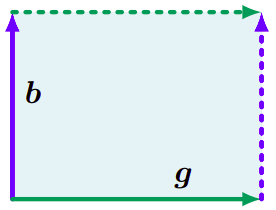
\includegraphics[
                width=\linewidth,
                height=3cm,
                keepaspectratio,
            ]{images/maths-for-ml/determinant-2d.png}
            \caption*{
                The area of the parallelogram (shaded region) spanned by the vectors $\bm{b}$ and $\bm{g}$ is $\dabs{\det([\bm{b}, \bm{g}])}$.
                \cite{mfml/book/mml/Deisenroth-Faisal-Ong}
            }
        \end{figure}
    \end{minipage}
    \hfill
    \begin{minipage}{0.45\linewidth}
        \begin{figure}[H]
            \centering
            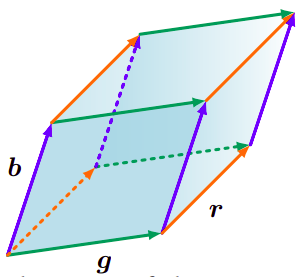
\includegraphics[
                width=\linewidth,
                height=3cm,
                keepaspectratio,
            ]{images/maths-for-ml/determinant-3d.png}
            \caption*{
                The volume of the parallelepiped (shaded volume) spanned by vectors $\bm{r}$, $\bm{b}$, $\bm{g}$ is $\dabs{\det([\bm{r}, \bm{b}, \bm{g}])}$.
                \cite{mfml/book/mml/Deisenroth-Faisal-Ong}
            }
        \end{figure}
    \end{minipage}
    \hfill
\end{table}


.\hfill
$
    \det(\bm{A}) 
    = \dabs{\bm{A}}
    = \begin{vmatrix}
        a_{11} & a_{12} & \cdots & a_{1n} \\
        a_{21} & a_{22} & \cdots & a_{2n} \\
        \vdots & \vdots & \ddots & \vdots \\
        a_{n1} & a_{n2} & \cdots & a_{nn} \\
    \end{vmatrix}
$
\hfill \cite{mfml/book/mml/Deisenroth-Faisal-Ong}

\begin{enumerate}
    \item 
    \begin{definition}[Determinant]
        A determinant is a mathematical object in the analysis and solution of systems of linear equations.
        \hfill \cite{mfml/book/mml/Deisenroth-Faisal-Ong}
    \end{definition}

    \item Determinants are \textbf{only} defined for square matrices $\bm{A} \in \mbbR^{n\times n}$ ,i.e., matrices with the same number of rows and columns.
    \hfill \cite{mfml/book/mml/Deisenroth-Faisal-Ong}

    \item The determinant of a square matrix $\bm{A} \in \mbbR^{n\times n}$ is a function that maps $\bm{A}$ onto a real number.
    \hfill \cite{mfml/book/mml/Deisenroth-Faisal-Ong}

    \item For $n=1$, $\det(\bm{A}) = \det(a_{11}) = a_{11}$
    \hfill \cite{mfml/book/mml/Deisenroth-Faisal-Ong}

    \item For $n=2$, 
    $
        \det(\bm{A}) 
        = \begin{vmatrix}
            a_{11} & a_{12} \\
            a_{21} & a_{22}
        \end{vmatrix} 
        = a_{11} a_{22} - a_{12} a_{21}
    $
    \hfill \cite{mfml/book/mml/Deisenroth-Faisal-Ong}

    \item  
    \begin{definition}[Determinant: Sarrus’ Rule]
        For $n=3$, 
        \hfill \cite{mfml/book/mml/Deisenroth-Faisal-Ong}
        \\[0.3cm]
        $
            \det(\bm{A}) 
            = \begin{vmatrix}
                a_{11} & a_{12} & a_{13} \\
                a_{21} & a_{22} & a_{23} \\
                a_{31} & a_{32} & a_{33} \\
            \end{vmatrix} 
            = a_{11} a_{22} a_{33}  + a_{21} a_{32} a_{13}  + a_{31} a_{12} a_{23}  - a_{31} a_{22} a_{13}  - a_{11} a_{32} a_{23}  - a_{21} a_{12} a_{33} 
        $
        \hfill \cite{mfml/book/mml/Deisenroth-Faisal-Ong}
    \end{definition}

    \item For a triangular matrix $\bm{T} \in \mbbR^{n\times n}$ , the determinant is the product of the diagonal elements, i.e., $\det(\bm{T}) = \dsum ^n _{i=1} \bm{T}_{ii}$
    \hfill \cite{mfml/book/mml/Deisenroth-Faisal-Ong}

    \item the determinant $\det(\bm{A})$ is the signed volume of an n-dimensional parallelepiped formed by columns of the matrix $\bm{A}$.
    \hfill \cite{mfml/book/mml/Deisenroth-Faisal-Ong}

    \item The sign of the determinant indicates the orientation of the spanning vectors.
    \hfill \cite{mfml/book/mml/Deisenroth-Faisal-Ong}

    \item 
    \begin{theorem}[Determinant: Laplace Expansion]
    Consider a matrix $\bm{A} \in \mbbR^{n\times n}$. Then, for all $j = 1, \cdots , n$:
    \hfill \cite{mfml/book/mml/Deisenroth-Faisal-Ong}
    \end{theorem}
    \begin{enumerate}
        \item Expansion along column $j$: 
        $
            \det(\bm{A}) = \dsum^n _{k=1} (-1)^{k+j}\  a_{kj}\ \det(\bm{A}_{k,j} )
        $
        \hfill \cite{mfml/book/mml/Deisenroth-Faisal-Ong}

        \item Expansion along row $j$:
        $
            \det(\bm{A}) = \dsum^n _{k=1} (-1)^{k+j}\  a_{jk}\ \det(\bm{A}_{j,k} )
        $
        \hfill \cite{mfml/book/mml/Deisenroth-Faisal-Ong}

        \item $\bm{A}_{k,j} \in \mbbR^{(n-1)\times(n-1)}$ is the sub-matrix of $\bm{A}$ that we obtain when deleting row $k$ and column $j$.
        \hfill \cite{mfml/book/mml/Deisenroth-Faisal-Ong}

        \item $\det(\bm{A}_{k,j} )$ is called a \textbf{minor} and $(-1)^{k+j}\ \det(\bm{A}_{k,j} )$ a \textbf{cofactor}.
        \hfill \cite{mfml/book/mml/Deisenroth-Faisal-Ong}
    \end{enumerate}

    \item \begin{theorem}[Determinant: product of eigenvalues]
        The determinant of a matrix $\bm{A} \in \mbbR^{n\times n}$ is the product of its eigenvalues, i.e.,
        \hfill \cite{mfml/book/mml/Deisenroth-Faisal-Ong}
        \\
        .\hfill
        $
            \det(\bm{A}) = \dprod_{i=1}^{n} \lambda_i
        $
        \hfill \cite{mfml/book/mml/Deisenroth-Faisal-Ong}
        \\
        where $\lambda_i \in \mathbb{C}$ are (possibly repeated) eigenvalues of $\bm{A}$.
        \hfill \cite{mfml/book/mml/Deisenroth-Faisal-Ong}
    \end{theorem}

\end{enumerate}



\begin{lstlisting}[
    language=Python,
    caption=Determinant of matrix - numPy
]
import numpy as np

# Define a square matrix
A = np.array([
    [1, 2],
    [3, 4]
])

# Compute the determinant
det_A = np.linalg.det(A)

print("Matrix A:\n", A)
print("Determinant of A:", det_A)
\end{lstlisting}




\subsubsection{Properties of Determinant}

For $\bm{A} \in \mbbR^{n\times n}$ the determinant exhibits the following properties:
\hfill \cite{mfml/book/mml/Deisenroth-Faisal-Ong}

\begin{enumerate}
    \item The determinant of a matrix product is the product of the corresponding determinants, $\det(\bm{AB}) = \det(\bm{A})\det(\bm{B})$.
    \hfill \cite{mfml/book/mml/Deisenroth-Faisal-Ong}

    \item Determinants are invariant to transposition, i.e., $\det(\bm{A}) = \det(\bm{A}^\top)$.
    \hfill \cite{mfml/book/mml/Deisenroth-Faisal-Ong}

    \item If $\bm{A}$ is regular (invertible), then $\det(\bm{A} ^{-1} ) = \dfrac{1} {\det(\bm{A})}$.
    \hfill \cite{mfml/book/mml/Deisenroth-Faisal-Ong}

    \item Similar matrices possess the same determinant. 
    Therefore, for a linear mapping $\Phi : V \to V$ all transformation matrices $\bm{A}_\Phi$ of $\Phi$ have the same determinant. 
    Thus, the determinant is invariant to the choice of basis of a linear mapping.
    \hfill \cite{mfml/book/mml/Deisenroth-Faisal-Ong}

    \item Adding a multiple of a column/row to another one does not change $\det(\bm{A})$.
    \hfill \cite{mfml/book/mml/Deisenroth-Faisal-Ong}

    \item Multiplication of a column/row with $\lambda \in \mbbR$ scales $\det(\bm{A})$ by $\lambda$. 
    In particular, $\det(\lambda \bm{A}) = \lambda^ n \ \det(\bm{A})$.
    \hfill \cite{mfml/book/mml/Deisenroth-Faisal-Ong}

    \item Swapping two rows/columns changes the sign of $\det(\bm{A})$.
    \hfill \cite{mfml/book/mml/Deisenroth-Faisal-Ong}

    \item[] \textbf{Note}: Because of the last three properties, we can use Gaussian elimination to compute $\det(\bm{A})$ by bringing $\bm{A}$ into row-echelon form. 
    We can stop Gaussian elimination when we have $\bm{A}$ in a triangular form where the elements below the diagonal are all $0$. 
    (the determinant of a triangular matrix is the product of the diagonal elements)
\end{enumerate}










\subsection{Trace ($\tr(A)$)}


\begin{lstlisting}[
    language=Python,
    caption=Trace of a matrix - numPy
]
import numpy as np

# Define a square matrix
A = np.array([
    [1, 2, 3],
    [4, 5, 6],
    [7, 8, 9]
])

# Compute the trace (sum of diagonal elements)
trace_A = np.trace(A)

print("Matrix A:\n", A)
print("Trace of A:", trace_A)
\end{lstlisting}

\begin{enumerate}
    \item
    \begin{definition}[Trace]
        The trace of a square matrix $\bm{A} \in \mbbR^{n\times n}$ is defined as $\tr(\bm{A}) := \dsum^n _{i=1} a_{ii}$ i.e. , the trace is the \textbf{sum of the diagonal elements} of $\bm{A}$.
        \hfill \cite{mfml/book/mml/Deisenroth-Faisal-Ong}
    \end{definition}

    \item
    \begin{theorem}[Trace: sum of eigenvalues]
        The trace of a matrix $\bm{A} \in \mbbR^{n\times n}$ is the sum of its eigenvalues, i.e.,
        \hfill \cite{mfml/book/mml/Deisenroth-Faisal-Ong}
        \\
        .\hfill
        $
            \det(\bm{A}) = \dsum_{i=1}^{n} \lambda_i
        $
        \hfill \cite{mfml/book/mml/Deisenroth-Faisal-Ong}
        \\
        where $\lambda_i \in \mathbb{C}$ are (possibly repeated) eigenvalues of $\bm{A}$.
        \hfill \cite{mfml/book/mml/Deisenroth-Faisal-Ong}
    \end{theorem}
\end{enumerate}


\subsubsection{Properties of Trace}

\begin{enumerate}
    \item $\tr(\bm{A} + \bm{B}) = \tr(\bm{A}) + \tr(\bm{B})$ for $\bm{A}, \bm{B} \in \mbbR^{n\times n}$
    \hfill \cite{mfml/book/mml/Deisenroth-Faisal-Ong}

    \item $\tr(\alpha \bm{A}) = \alpha\ \tr(\bm{A}), \alpha \in \mbbR$ for $\bm{A} \in \mbbR^{n\times n}$
    \hfill \cite{mfml/book/mml/Deisenroth-Faisal-Ong}

    \item $\tr(\bm{I}_n) = n$
    \hfill \cite{mfml/book/mml/Deisenroth-Faisal-Ong}

    \item $\tr(\bm{AB}) = \tr(\bm{BA})$ for $\bm{A} \in \mbbR^{n\times k}, \bm{B} \in \mbbR^{k\times n}$
    \hfill \cite{mfml/book/mml/Deisenroth-Faisal-Ong}

    \item The trace is invariant under cyclic permutations, ie, $\tr(\bm{AKL}) = \tr(\bm{KLA})$ for matrices $\bm{A} \in  \mbbR^{a \times k}, \bm{K} \in  \mbbR^{k \times l}, \bm{L} \in  \mbbR^{l \times a}$.
    \hfill \cite{mfml/book/mml/Deisenroth-Faisal-Ong}

    \item $
        \tr(\bm{xy}^\top) = \tr(\bm{y} ^\top \bm{x}) = \bm{y} ^\top \bm{x} \in \mbbR\
        \forall \bm{x}, \bm{y} \in \mbbR^n
    $
    \hfill \cite{mfml/book/mml/Deisenroth-Faisal-Ong}

    \item Given $\Phi : V \to V$, then $\tr(\Phi) = \tr(\bm{A}_\Phi)$. while matrix representations of linear mappings are basis dependent the trace of a linear mapping $\Phi$ is independent of the basis.
    \hfill \cite{mfml/book/mml/Deisenroth-Faisal-Ong}
\end{enumerate}








\subsection{Characteristic Polynomial ($p_A(\lambda)$)}

\begin{enumerate}
    \item 
    \begin{definition}[Characteristic Polynomial]
        For $\lambda \in \mbbR$ and a square matrix $\bm{A} \in \mbbR^{n\times n}$:
        \\
        $
            \begin{aligned}
                p_{\bm{A}}(\lambda ) &:= \det(\bm{A} - \lambda \bm{I}) \\
                &= c_0 + c_1\lambda  + c_2\lambda  ^2 + \cdots + c_{n-1}\lambda ^{( n-1)} + (-1)^n\lambda^  n
            \end{aligned}
        $
        \\
        $c_0, \cdots , c_{n-1} \in \mbbR$, is the characteristic polynomial of $\bm{A}$.
    \end{definition}

    \item $c_0 = \det(\bm{A}), c_{n-1} = (-1)^{n-1}\ \tr(\bm{A})$
\end{enumerate}










\subsection{Eigenvalues ($\lambda$) \& Eigenvectors}

\begin{enumerate}
    \item Eigen is a German word meaning “characteristic”, “self”, or “own”.
    \hfill \cite{mfml/book/mml/Deisenroth-Faisal-Ong}

    \item \textbf{Definition}: Let $\bm{A} \in \mathbb{R}^{n\times n}$ be a square matrix. 
    Then $\lambda \in \mathbb{R}$ is an eigenvalue of $\bm{A}$ and $\bm{x} \in \mathbb{R}^n\backslash\dCurlyBrac{0}$ is the corresponding eigenvector of $\bm{A}$ if
    $\bm{Ax} = \lambda \bm{x}$.
    \hfill \cite{mfml/book/mml/Deisenroth-Faisal-Ong}

    \item $\bm{Ax} = \lambda \bm{x}$ is called eigenvalue equation.
    \hfill \cite{mfml/book/mml/Deisenroth-Faisal-Ong}

    \item it is often a convention that eigenvalues are sorted in descending order, so that the largest eigenvalue and associated eigenvector are called the \textbf{first eigenvalue} and its associated eigenvector, and the second largest called the \textbf{second eigenvalue} and its associated eigenvector, and so on.
    \hfill \cite{mfml/book/mml/Deisenroth-Faisal-Ong}

    \item The following statements are equivalent:
    \begin{enumerate}
        \item $\lambda$ is an eigenvalue of $\bm{A} \in \mathbb{R}^{n\times n}$
        \hfill \cite{mfml/book/mml/Deisenroth-Faisal-Ong}

        \item There exists an $\bm{x} \in \mathbb{R}^n\backslash\dCurlyBrac{0}$ with $\bm{Ax} = \lambda \bm{x}$, or equivalently, $(\bm{A} - \lambda \bm{I}_n)\bm{x} = 0$ can be solved non-trivially, i.e., $\bm{x} \neq 0$.
        \hfill \cite{mfml/book/mml/Deisenroth-Faisal-Ong}

        \item $rk(\bm{A} - \lambda \bm{I}_n) < n$
        \hfill \cite{mfml/book/mml/Deisenroth-Faisal-Ong}

        \item $\det(\bm{A} - \lambda \bm{I}_n) = 0$
        \hfill \cite{mfml/book/mml/Deisenroth-Faisal-Ong}
    \end{enumerate}

    \item \textbf{Non-uniqueness of eigenvectors}: If $\bm{x}$ is an eigenvector of $\bm{A}$ associated with eigenvalue $\lambda$, then for any $c \in \mathbb{R}\backslash \dCurlyBrac{0}$ it holds that $c\bm{x}$ is an eigenvector of $\bm{A}$ with the same eigenvalue since $\bm{A}(c\bm{x}) = c\bm{Ax} = c\lambda\bm{x} = \lambda(c\bm{x})$. All vectors that are collinear to $\bm{x}$ are also eigenvectors of $\bm{A}$.
    \hfill \cite{mfml/book/mml/Deisenroth-Faisal-Ong}

    \item \textbf{Theorem}: $\lambda  \in \mathbb{R}$ is an eigenvalue of $\bm{A} \in \mathbb{R}^{n\times n}$ if and only if $\lambda$  is a root of the characteristic polynomial $p_{\bm{A}}(\lambda )$ of $\bm{A}$.
    \hfill \cite{mfml/book/mml/Deisenroth-Faisal-Ong}

    \item \textbf{Definition}: Let a square matrix $\bm{A}$ have an eigenvalue $\lambda_i$ . 
    The \textbf{algebraic  multiplicity} of $\lambda_i$ is the number of times the root appears in the characteristic polynomial.
    \hfill \cite{mfml/book/mml/Deisenroth-Faisal-Ong}

    \item \textbf{Definition}: Let $\lambda_i$ be an eigenvalue of a square matrix $\bm{A}$. 
    Then the \textbf{geometric multiplicity} of $\lambda_i$ is the number of linearly independent eigenvectors associated with $\lambda_i$. 
    In other words, it is the dimensionality of the eigenspace spanned by the eigenvectors associated with $\lambda_i$.
    \hfill \cite{mfml/book/mml/Deisenroth-Faisal-Ong}

    \item A specific eigenvalue’s geometric multiplicity must be at least one because every eigenvalue has at least one associated eigenvector. 
    An eigenvalue’s geometric multiplicity cannot exceed its algebraic multiplicity, but it may be lower.

    \item Geometrically, the eigenvector corresponding to a nonzero eigenvalue points in a direction that is stretched by the linear mapping.
    The eigenvalue is the factor by which it is stretched. 
    If the eigenvalue is negative, the direction of the stretching is flipped.
    \hfill \cite{mfml/book/mml/Deisenroth-Faisal-Ong}

    \item \textbf{The Case of the Identity Matrix}: The identity matrix $\bm{I} \in \mathbb{R}^{n\times n}$ has characteristic polynomial $p_{\bm{I}} (\lambda ) = \det(\bm{I} -\lambda \bm{I}) = (1-\bm{\lambda }) ^n = 0$, which has only one eigenvalue $\lambda  = 1$ that occurs $n$ times. 
    Moreover, $\bm{Ix} = \lambda \bm{x} = 1\bm{x}$ holds for all vectors $\bm{x} \in \mathbb{R}^n\backslash \dCurlyBrac{0}$. 
    Because of this, the sole eigenspace $E_1$ of the identity matrix spans $n$ dimensions, and all $n$ standard basis vectors of $\mathbb{R}^n$ are eigenvectors of $\bm{I}$.
    \hfill \cite{mfml/book/mml/Deisenroth-Faisal-Ong}

    \item \textbf{Theorem}: The eigenvectors $\bm{x}_1, \cdots , \bm{x}_n$ of a matrix $\bm{A} \in \mathbb{R}^{n\times n}$ with $n$ distinct eigenvalues $\lambda _1, \cdots , \lambda _n$ are linearly independent.
    This theorem states that eigenvectors of a matrix with $n$ distinct eigenvalues form a basis of $\mathbb{R}^n$.
    \hfill \cite{mfml/book/mml/Deisenroth-Faisal-Ong}

    \item 
\end{enumerate}




\begin{lstlisting}[
    language=Python,
    caption=Eigenvalues \& Eigenvectors of a Matrix - numPy
]
import numpy as np

# Define a square matrix
A = np.random.randint(-10, 10, size=(3,3), dtype=int)
print(A)

# Compute eigenvalues and eigenvectors
# eigenvalues: 1D array of eigenvalues.
# eigenvectors: 2D array where each column is an eigenvector.
eigenvalues, eigenvectors = np.linalg.eig(A)
print(eigenvalues)
print(eigenvectors)
\end{lstlisting}



\subsubsection{Properties of eigenvalues \& eigenvectors}

\begin{enumerate}
    \item A matrix $\bm{A}$ and its transpose $\bm{A}^\top$ possess the same eigenvalues, but not necessarily the same eigenvectors.
    \hfill \cite{mfml/book/mml/Deisenroth-Faisal-Ong}

    \item Similar matrices possess the same eigenvalues.
    Therefore, a linear mapping $\Phi$ has eigenvalues that are independent of the choice of basis of its transformation matrix.
    \hfill \cite{mfml/book/mml/Deisenroth-Faisal-Ong}

    \item Symmetric, positive definite (SPD) matrices \textbf{always} have positive, real eigenvalues.
    \hfill \cite{mfml/book/mml/Deisenroth-Faisal-Ong}
\end{enumerate}




\subsection{Eigenspace ($E_\lambda $) \& Eigenspectrum}

\begin{enumerate}
    \item \textbf{Definition}: For $\bm{A} \in \mathbb{R}^{n\times n}$ , the set of all eigenvectors of $\bm{A}$ associated with an eigenvalue $\lambda $ spans a subspace of $\mathbb{R}^n$, which is called the \textbf{eigenspace} of $\bm{A}$ with respect to $\lambda $ and is denoted by $E_\lambda $.
    \hfill \cite{mfml/book/mml/Deisenroth-Faisal-Ong}

    \item \textbf{Definition}: The set of all eigenvalues of $\bm{A}$ is called the \textbf{eigenspectrum}, or just spectrum, of $\bm{A}$.
    \hfill \cite{mfml/book/mml/Deisenroth-Faisal-Ong}

    \item If $\lambda $ is an eigenvalue of $\bm{A} \in \mathbb{R}^{n\times n}$ , then the corresponding eigenspace $E_\lambda $ is the solution space of the homogeneous system of linear equations $(\bm{A} - \lambda \bm{I})\bm{x} = 0$.
    \hfill \cite{mfml/book/mml/Deisenroth-Faisal-Ong}
\end{enumerate}


\subsubsection{Properties of Eigenspace \& Eigenspectrum}

\begin{enumerate}
    \item The eigenspace $E_\lambda$  is the null space of $\bm{A} - \lambda \bm{I}$ since:
    \hfill \cite{mfml/book/mml/Deisenroth-Faisal-Ong}
    \\
    .\hfill
    $
        \begin{aligned}
            \bm{Ax} = \lambda \bm{x}
            & \Longleftrightarrow \bm{Ax} - \lambda \bm{x} = 0 \\
            & \Longleftrightarrow (\bm{A} - \lambda \bm{I})\bm{x} = 0  
            & \Longleftrightarrow \bm{x} \in \ker(\bm{A} - \lambda \bm{I})
        \end{aligned}
    $
    \hfill \cite{mfml/book/mml/Deisenroth-Faisal-Ong}
\end{enumerate}










\section{Matrix Decomposition/Factorization}
\subsection{Cholesky Decomposition ($A=LL^\top$)}

\begin{enumerate}
    \item 
    \begin{theorem}[Cholesky Decomposition]
        A symmetric, positive definite matrix $\bm{A}$ can be factorized into a product $\bm{A} = \bm{LL}^\top$, where L is a lower-triangular matrix with positive diagonal elements:
        \hfill \cite{mfml/book/mml/Deisenroth-Faisal-Ong}
        \\
        .\hfill
        $
            \underset
            {
                \displaystyle
                \bm{A}
            } 
            {\underbrace{
                \displaystyle
                \begin{bmatrix}
                    a_{11} & \cdots & a_{1n} \\
                    \vdots & \ddots & \vdots \\
                    a_{n1} & \cdots & a_{nn}
                \end{bmatrix}
            }}
            =
            \underset
            {
                \displaystyle
                \bm{L}
            } 
            {\underbrace{
                \displaystyle
                \begin{bmatrix}
                    l_{11} & \cdots & 0 \\
                    \vdots & \ddots & \vdots \\
                    l_{n1} & \cdots & l_{nn}
                \end{bmatrix}
            }}
            \underset
            {
                \displaystyle
                \bm{L}^\top
            } 
            {\underbrace{
                \displaystyle
                \begin{bmatrix}
                    l_{11} & \cdots & l_{n1} \\
                    \vdots & \ddots & \vdots \\
                    0 & \cdots & l_{nn}
                \end{bmatrix}
            }}
        $
        \hfill \cite{mfml/book/mml/Deisenroth-Faisal-Ong}
        \\
        $\bm{L}$ is called the \textbf{Cholesky factor} of $\bm{A}$, and $\bm{L}$ is unique.
        \hfill \cite{mfml/book/mml/Deisenroth-Faisal-Ong}
    \end{theorem}

    \item In machine learning, symmetric positive definite matrices require frequent manipulation, e.g., the covariance matrix of a multivariate Gaussian variable is symmetric, positive definite. 
    The Cholesky factorization of this covariance matrix allows us to generate samples from a Gaussian distribution.
    \hfill \cite{mfml/book/mml/Deisenroth-Faisal-Ong}

    \item  It also allows us to perform a linear transformation of random variables, which is heavily exploited when computing gradients in deep stochastic models, such as the variational auto-encoder.
    \hfill \cite{mfml/book/mml/Deisenroth-Faisal-Ong}

    \item The Cholesky decomposition also allows us to compute determinants very efficiently: 
    $
        \det(\bm{A}) 
        = \det(\bm{L}) \det(\bm{L}^\top) 
        = \det(\bm{L})^2
        = \dprod_i l_{ii}^2
    $
    \hfill \cite{mfml/book/mml/Deisenroth-Faisal-Ong}
\end{enumerate}


\begin{lstlisting}[
    language=Python,
    caption=Cholesky Decomposition - numPy
]
import numpy as np

# generate a random matrix
A = np.random.randint(-10, 10, size=(3,3))
# Create a symmetric positive definite matrix
A = A.T @ A

# Perform Cholesky decomposition
L = np.linalg.cholesky(A)

print("Matrix A:")
print(A)
print("\nCholesky factor L:")
print(L)
\end{lstlisting}








\subsection{Eigendecomposition ($A = P DP ^{-1}$)}

\begin{figure}[H]
    \centering
    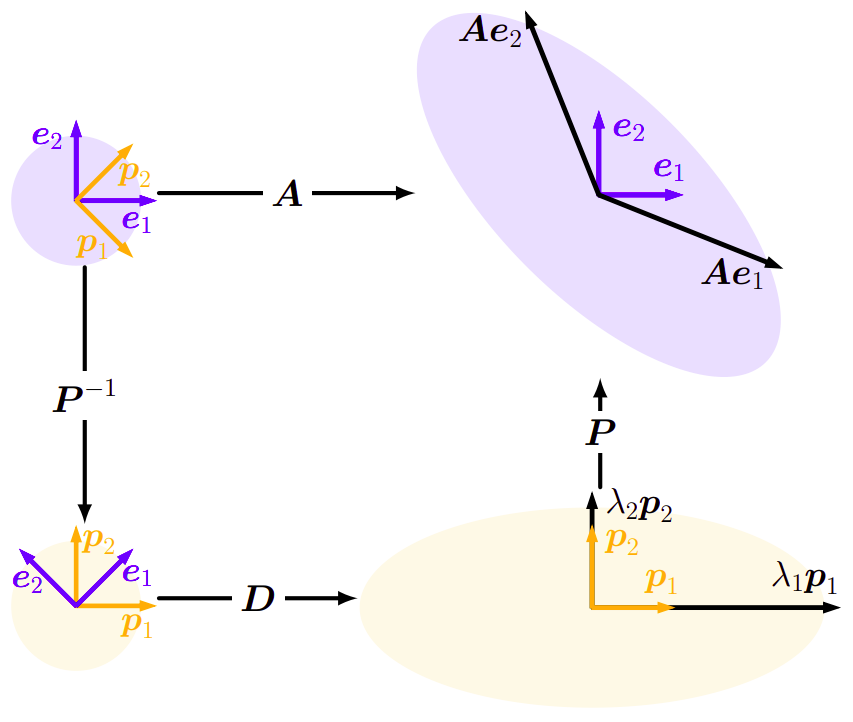
\includegraphics[
        width=\linewidth,
        height=5cm,
        keepaspectratio,
    ]{images/maths-for-ml/eigendecomposition.png}
    \caption*{
        Intuition behind the eigendecomposition as sequential transformations.
        \\
        \textbf{Top-left to bottom-left}: $\bm{P}^{-1}$ performs a basis change (here drawn in $\mathbb{R}^2$ and depicted as a rotation-like operation) from the standard basis into the eigenbasis.
        \\
        \textbf{Bottom-left to bottom-right}: $\bm{D}$ performs a scaling along the remapped orthogonal eigenvectors, depicted here by a circle being stretched to an ellipse. 
        \\
        \textbf{Bottom-right to top-right}: $\bm{P}$ undoes the basis change (depicted as a reverse rotation) and restores the original coordinate frame.
    }
\end{figure}


\begin{enumerate}
    \item 
    \begin{theorem}[Eigendecomposition]
        A square matrix $\bm{A} \in \mathbb{R}^{n\times n}$ can be factored into $\bm{A} = \bm{PDP}^{-1}$ where $\bm{P} \in \mathbb{R}^{n\times n}$ and $\bm{D}$ is a diagonal matrix whose diagonal entries are the eigenvalues of $\bm{A}$, if and only if the eigenvectors of $\bm{A}$ form a basis of $\mathbb{R}^n$.
        \hfill \cite{mfml/book/mml/Deisenroth-Faisal-Ong}
    \end{theorem}

    \item \textbf{Steps}:
    \begin{enumerate}
        \item Compute eigenvalues and eigenvectors

        \item Check for existence (eigenvectors span $\mathbb{R}^n$ or not)

        \item Construct the matrix P to diagonalize A
        \begin{enumerate}
            \item $\bm{P} = [\bm{p}_1, \cdots, \bm{p}_n]$

            \item $\bm{D} = \bm{P}^{-1}\bm{AP} = \bm{P}^{\top}\bm{AP}$
            \hfill (if $\bm{A}$ is symmetric, $\bm{P}^{-1} = \bm{P}^{\top}$)
        \end{enumerate}
    \end{enumerate}

    \item we can find a matrix power for a matrix $\bm{A} \in \mathbb{R}^{n\times n}$ via the eigenvalue decomposition (if it exists) so that:
    \hfill \cite{mfml/book/mml/Deisenroth-Faisal-Ong}
    \\
    .\hfill
    $
        \bm{A}^k 
        = (\bm{PDP}^{-1})^k 
        = \bm{PDP}^{-1}\bm{PDP}^{-1}\cdots \bm{PDP}^{-1} 
        = \bm{PD}^k \bm{P}^{-1}
    $
    \hfill \cite{mfml/book/mml/Deisenroth-Faisal-Ong}

    \item Assume that the eigendecomposition $\bm{A} = (\bm{PDP}^{-1})$ exists. Then: 
    \hfill \cite{mfml/book/mml/Deisenroth-Faisal-Ong}
    \\
    .\hfill
    $
        \det(\bm{A}) 
        = \det(\bm{PDP}^{ -1}) 
        = \det(\bm{P}) \det(\bm{D}) \det(\bm{P}^{-1})
        = \det(\bm{D})
        = \dprod_{i} d_{ii}
    $
    \hfill \cite{mfml/book/mml/Deisenroth-Faisal-Ong}

    \item eigendecomposition operates within the same vector space, where the same basis change is applied and then undone. 
    \hfill \cite{mfml/book/mml/Deisenroth-Faisal-Ong}
\end{enumerate}



\begin{lstlisting}[
    language=Python,
    caption=Eigendecomposition - numPy
]
import numpy as np

# Define a square matrix
A = np.array([[4, -2],
              [1,  1]])

# Perform eigendecomposition
eigenvalues, eigenvectors = np.linalg.eig(A)

# Construct D and P
D = np.diag(eigenvalues)
P = eigenvectors

# Inverse of P
P_inv = np.linalg.inv(P)

# Reconstruct A
A_reconstructed = P @ D @ P_inv

# Print results
print("Original matrix A:")
print(A)

print("\nEigenvalues (D):")
print(D)

print("\nEigenvectors (P):")
print(P)

print("\nReconstructed A (P D P_inv):")
print(A_reconstructed)

print("\nCheck reconstruction accuracy:", np.allclose(A, A_reconstructed))
\end{lstlisting}







\subsection{Singular Value Decomposition (SVD) ($A = U \Sigma V^\top$)}


\begin{figure}[H]
    \centering
    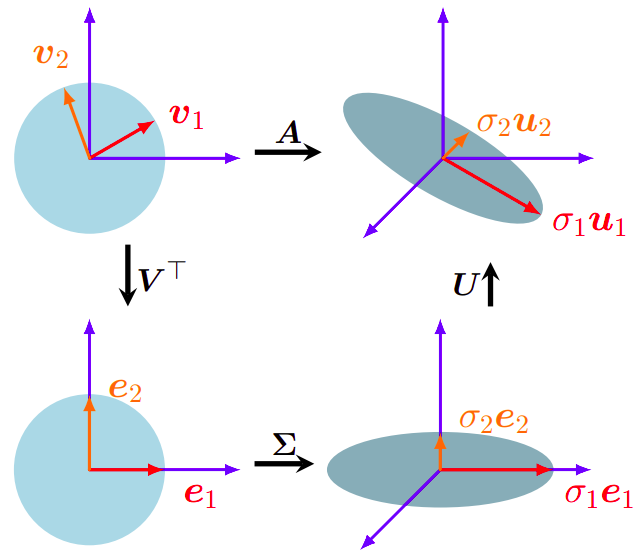
\includegraphics[
        width=\linewidth,
        height=5cm,
        keepaspectratio,
    ]{images/maths-for-ml/singular-value-decomposition.png}
    \caption*{
        Intuition behind the SVD of a matrix $\bm{A} \in \mathbb{R}^{3\times 2}$ as sequential transformations.
        \\
        \textbf{Top-left to bottom-left}: $\bm{V}^\top$ performs a basis change in $\mathbb{R}^2$.
        \\
        \textbf{Bottom-left to bottom-right}: $\Sigma$ scales and maps from $\mathbb{R}^2$ to $\mathbb{R}^3$ . The ellipse in the bottom-right lives in $\mathbb{R}^3$. The third dimension is orthogonal to the surface of the elliptical disk.
        \\
        \textbf{Bottom-right to top-right}: $\bm{U}$ performs a basis change within $\mathbb{R}^3$.
    }
\end{figure}


\begin{enumerate}
    \item The singular value decomposition (SVD) of a matrix is a central matrix decomposition method in linear algebra.
    \hfill \cite{mfml/book/mml/Deisenroth-Faisal-Ong}

    \item It has been referred to as the “fundamental theorem of linear algebra” because it can be applied to \textbf{all matrices}, not only to square matrices, and it \textbf{always exists}.
    \hfill \cite{mfml/book/mml/Deisenroth-Faisal-Ong}

    \item the SVD of a matrix $\bm{A}$, which represents a linear mapping $\Phi : V \to W$, quantifies the change between the underlying geometry of these two vector spaces.
    \hfill \cite{mfml/book/mml/Deisenroth-Faisal-Ong}

    \item 
    \begin{theorem}[SVD Theorem]
        Let $\bm{A} \in \mathbb{R}^{m\times n}$ be a rectangular matrix of rank $r \in [0,\ \min(m, n)]$. 
        The SVD of $\bm{A}$ is a decomposition of the form 
        $
            \underset{\displaystyle m\times n}{\underbrace{\bm{A}}} = 
            \underset{\displaystyle m\times m}{\underbrace{\bm{U}}}\ 
            \underset{\displaystyle m\times n}{\underbrace{\bm{\Sigma}}}\ 
            \underset{\displaystyle n\times n}{\underbrace{\bm{V}^\top}}
        $ 
        with an orthogonal matrix $\bm{U} \in \mathbb{R}^{m\times m}$ with column vectors $\bm{u}_i$ , $i = 1, \cdots , m$, and an orthogonal matrix $\bm{V} \in \mathbb{R}^{n\times n}$ with column vectors $\bm{v}_j$ , $j = 1, \cdots , n$.
        Moreover, $\bm{\Sigma}$ is an $m \times n$ matrix with $\Sigma_{ii} = \sigma_i \geq 0$ and $\Sigma_{ij} = 0, i \neq j$.
        \hfill \cite{mfml/book/mml/Deisenroth-Faisal-Ong}
    \end{theorem}
\end{enumerate}

























